\documentclass{beamer}
\usepackage{beamerthemesplit, graphicx}
\usetheme{VAXMAN}
%
\title{QNICE -- a nice 16 bit architecture\\~\\ISA v. 1.7}
\author{Bernd Ulmann}
%\date{}
\begin{document}
 \begin{frame}
  \titlepage
 \end{frame}
%
% \section{Introduction}
%  \subsection{Goal}
   \begin{frame}
    \frametitle{Goal}
    Why a new 16 bit processor architecture? Why not stay with commodity
    products and a wider bus width?
    \begin{itemize}
     \item First of all, there is nothing like developing your own CPU
      from scratch -- nothing!
     \item The QNICE architecture was developed during 2006 with its
      32 bit predecessor NICE (cf. \cite{nice} and \cite{nice_html}) in
      mind. 
     \item The 16 bit data bus width was chosen to ease an actual 
      implementation of the processor either using TTL chips as in many
      other homebrew CPU projects\footnote{Most notably Bill Buzbee's
      Magic, cf \cite{magic}.} or using more modern FPGAs with a bit
      of surrounding circuitry.
     \item Thanks to Mirko Holzer the project was revived in 2015, 
      first with an AVR-implementation and then with a FPGA-version of
      this processor.
    \end{itemize}
   \end{frame}
%
%  \subsection{Basics}
   \begin{frame}
    \frametitle{Basics}
    \begin{itemize}
     \item 16 bit data and address bus width (little endian!)
     \item Rather fixed instruction format -- every instruction occupies
      one 16 bit machine word
     \item 16 general purpose registers divided into two banks of eight
      registers each
     \item The register bank containing registers 0\dots 7 is actually
      a window to a high speed RAM so in fact there are $256\times 8+8=2056$ 
      registers all in all
     \item moving the register window is accomplished in a single operation
      making push/pop operations virtually unnecessary
     \item Very small instruction set (23 instructions)
     \item 4 addressing modes
    \end{itemize}
   \end{frame}
%
% \section{Architecture}
%  \subsection{Registers}
   \begin{frame}
    \frametitle{Registers}
    \begin{itemize}
     \item At any moment of a program run there are 16 general purpose 
      registers visible to the program:
      \begin{center}
       \begin{tabular}{|c|c|c||c|c|c|c|c|}
        \hline
         {\tt R0}&\dots&{\tt R7}&{\tt R8}&\dots&{\tt R13}&{\tt R14}&{\tt R15}\\
        \hline
       \end{tabular}
      \end{center}
     \item Some registers serve a special function in the processor:
      \begin{description}
       \item [{\tt R13}:] Normally used as a stack pointer -- especially the
        subroutine call instructions use this register as a stack pointer
        (\texttt{SP}).
       \item [{\tt R14}:] Statusregister ({\tt SR} for short).
       \item [{\tt R15}:] Program counter (\texttt{PC}).
      \end{description}
     \item The upper eight registers {\tt R8}\dots{\tt R15} are always the
      same while the lower set of eight registers is a window
      into a $256\times 8$ register bank of 16 bit bus width.
    \end{itemize}
   \end{frame}
%
%  \subsection{The status register {\tt R14}}
   \begin{frame}
    \frametitle{The status register {\tt R14}}
    The status register is divided into two parts: The lower
    8 bits are the status bits reflecting the current processor
    state while the upper 8 bits ({\tt rbank}) are used to control 
    the register bank circuitry:
    \begin{center}
     \begin{tabular}{|c||c|c|c|c|c|c|c|c|}
      \hline
       {\tt rbank}&
       ---&---&{\tt V}&{\tt N}&{\tt Z}&{\tt C}&{\tt X}&{\tt 1}\\
      \hline
     \end{tabular}
    \end{center}
    \begin{description}
     \item [{\tt 1}:] Always set to 1
     \item [{\tt X}:] Used by shift instructions only.
     \item [{\tt C}:] Carry flag
     \item [{\tt Z}:] 1 if the last result was {\tt 0x0000}
     \item [{\tt N}:] 1 if the last result was negative
     \item [{\tt V}:] 1 if the last operation caused an overflow
%     \item [{\tt I}:] 1 if an interrupt occured
%     \item [{\tt M}:] If set to 1, maskable interrupts are allowed
    \end{description}
   \end{frame}
%
   \begin{frame}
%    \frametitle{The status register {\tt R14}}
    \begin{itemize}
     \item As already mentioned, the upper 8 bits of {\tt R14}, called
      {\tt rbank}, control the register bank circuitry.
     \item Since there are 256 times 8 registers available as 
      {\tt R0}\dots{\tt R7}, the eight bits of {\tt rbank} suffice to
      specify one out of these 256 pages as the actual register page
      to be used.
     \item To switch between register pages it is only necessary to 
      change the contents of {\tt rbank} -- normally this will be 
      accomplished by the {\tt INCRB} and {\tt DECRB} instructions.
     \item The multiple register banks are very handy in programming
      subroutines since they remove the necessity of saving lots of
      registers on entry and restoring them on exit of a subroutine.
    \end{itemize}
   \end{frame}
%
%  \subsection{Input/Output}
   \begin{frame}
    \frametitle{Input/Ouput}
    \begin{itemize}
     \item All input/output operations of QNICE take place through
      a memory mapped I/O system, so there are no special I/O instructions
      as some other processors feature.
     \item The upper 256 words of memory are reserved for I/O controllers
      which can be easily accessed using normal instructions with
      addressing modes referring to memory cells.
    \end{itemize}
   \end{frame}
%
% \section{Instruction set and addressing modes}
%  \subsection{Instruction set basics}
   \begin{frame}
    \frametitle{Instruction set basics}
    \begin{itemize}
     \item QNICE utilizes 18 basic instructions, all of which (apart
      from the control group, which takes one optional operand) are two 
      operand instructions. 
     \item Instructions like {\tt ADD R0, R1} will actually perform an
      operation like {\tt R1 := R1 + R0} -- the only exceptions being
      \begin{itemize}
       \item the two shift instructions {\tt SHL} and {\tt SHR} where the 
        first operand specifies the number of places to be shifted and
       \item the four jump and branch instructions {\tt ABRA}, {\tt ASUB},
        {\tt RBRA} and {\tt RSUB} which only take a 
        a destination and a condition code.
      \end{itemize}
     \item All operands, apart from the condition code of a jump or
      branch instruction, of course, can be specified using one out
      of four possible addressing modes ({\tt Rxx}, {\tt @Rxx}, {\tt @Rxx++} 
      and {\tt @--Rxx}).
    \end{itemize}
   \end{frame}
%
%  \subsection{Instruction format}
   \begin{frame}
    \frametitle{Instruction format}
    \begin{itemize}
     \item Most of QNICE's instructions feature a single instruction 
      format, the only exceptions are the four branch and jump instructions:
      \begin{center}
       \begin{tabular}{|c||c|c||c|c|}
        \hline
         4 bit&4 bit&2 bit&4 bit&2 bit\\
         {\tt opcode}&{\tt src rxx}&{\tt src mode}&
                      {\tt dst rxx}&{\tt dst mode}\\
        \hline
       \end{tabular}
      \end{center}
     \item The control instructions with opcode \texttt{E} have the 
      following general format:
      \begin{center}
       \begin{tabular}{|c||c||c|c|}
        \hline
         4 bit&6 bit&4 bit&2 bit\\
         {\tt opcode}&{\tt command}&{\tt dst rxx}&\texttt{dst mode}\\
        \hline
       \end{tabular}
      \end{center}
     \item The four jump and branch instructions use the following instruction
      format with mode bits \texttt{00}, \texttt{01}, \texttt{10},
      \texttt{11} specifying \texttt{ABRA}, \texttt{ASUB}, \texttt{RBRA}, 
      and \texttt{RSUB}:
      {\scriptsize
       \begin{center}
        \begin{tabular}{|c||c|c||c||c|c|}
         \hline
          4 bit&4 bit&2 bit&2 bit&1 bit&3 bit\\
               &     &     &     &{\tt negate}&{\tt select}\\
          {\tt opcode}&{\tt src rxx}&{\tt src mode}&
                       {\tt mode}&{\tt condition}&{\tt condition}\\
         \hline
        \end{tabular}
       \end{center}
      }
    \end{itemize}
   \end{frame}
%
%  \subsection{List of instructions}
   \begin{frame}
    \frametitle{List of instructions}
    \begin{center}
     \begin{tabular}{|c|ll|l|}
      \hline
       Opc&Instr&Operands&Effect\\
      \hline
       {\tt 0}&{\tt MOVE}&{\tt src, dst}&{\tt dst := src}\\
       {\tt 1}&{\tt ADD}&{\tt src, dst}&{\tt dst := dst + src}\\
       {\tt 2}&{\tt ADDC}&{\tt src, dst}&{\tt dst := dst + src + C}\\
       {\tt 3}&{\tt SUB}&{\tt src, dst}&{\tt dst := dst - src}\\
       {\tt 4}&{\tt SUBC}&{\tt src, dst}&{\tt dst := dst - src - C}\\
       {\tt 5}&{\tt SHL}&{\tt src, dst}&{\tt dst << src}, fill with X, shift to C\\
       {\tt 6}&{\tt SHR}&{\tt src, dst}&{\tt dst >> src}, fill with C, shift to X\\
       {\tt 7}&{\tt SWAP}&{\tt src, dst}&{\tt dst := ((src << 8) \& 0xFF00) |}\\
              &          &              &{\tt ((src >> 8) \& 0xFF)}\\
       {\tt 8}&{\tt NOT}&{\tt src, dst}&{\tt dst := !src}\\
      \hline
     \end{tabular}
    \end{center}
   \end{frame}
%
   \begin{frame}
    \frametitle{List of instructions}
    \begin{center}
     \begin{tabular}{|c|ll|l|}
      \hline
       Opc&Instr&Operands&Effect\\
      \hline
       {\tt 9}&{\tt AND}&{\tt src, dst}&{\tt dst := dst \& src}\\
       {\tt A}&{\tt OR}&{\tt src, dst}&{\tt dst := dst | src}\\
       {\tt B}&{\tt XOR}&{\tt src, dst}&{\tt dst := dst \^\ src}\\
       {\tt C}&{\tt CMP}&{\tt src, dst}&compare {\tt src} with {\tt dst}\\ 
       {\tt D}&&&reserved\\
       {\tt E}&{\tt HALT}&&Halt the processor\\
       {\tt E}&{\tt RTI}&&Return from interrupt\\
       {\tt E}&{\tt INT}&\texttt{dst}&Issue software interrupt\\
       {\tt E}&{\tt INCRB}&&Increment register bank addr.\\
       {\tt E}&{\tt DECRB}&&Decrement register bank addr.\\
       {\tt E}&{\tt EXC}&{\tt const, dst}&Exchange shadow register\\
       {\tt F}&{\tt ABRA}&{\tt src, [!]cond}&Absolute branch\\
       {\tt F}&{\tt ASUB}&{\tt src, [!]cond}&Absolut subroutine call\\
       {\tt F}&{\tt RBRA}&{\tt src, [!]cond}&Relative branch\\
       {\tt F}&{\tt RSUB}&{\tt src, [!]cond}&Relative subroutine call\\
      \hline
     \end{tabular}
    \end{center}
   \end{frame}
%
%  \subsection{Affected condition bits}
   \begin{frame}
    \frametitle{Affected condition bits}
    The following table shows which instructions (R)eads, (W)rites or is 
    (C)ontrolled by which condition bits:
    \begin{center}
     \begin{tabular}{|l|c|c|c|c|c|c|}
      \hline
       Instruction&\texttt{V}&\texttt{N}&\texttt{Z}&\texttt{C}&\texttt{X}&\texttt{1}\\
      \hline
       \texttt{MOVE} & &W&W& & & \\
       \texttt{ADD}  &W&W&W&W& & \\
       \texttt{ADDC} &W&W&W&R/W& & \\
       \texttt{SUB}  &W&W&W&W& & \\
       \texttt{SUBC} &W&W&W&R/W& & \\
       \texttt{SHL}  & &W&W&W&R& \\
       \texttt{SHR}  & &W&W&R&W& \\
       \texttt{SWAP} & &W&W& & & \\
       \texttt{NOT}  & &W&W& & & \\
       \texttt{AND}  & &W&W& & & \\
       \texttt{OR}   & &W&W& & & \\
       \texttt{XOR}  & &W&W& & & \\
      \hline
     \end{tabular}
    \end{center}
   \end{frame}
%
%  \subsection{Affected condition bits}
   \begin{frame}
    \frametitle{Affected condition bits}
    \begin{center}
     \begin{tabular}{|l|c|c|c|c|c|c|}
      \hline
       Instruction&\texttt{V}&\texttt{N}&\texttt{Z}&\texttt{C}&\texttt{X}&\texttt{1}\\
      \hline
       \texttt{CMP}  &W&W&W& & & \\
       \texttt{HALT} & & & & & & \\
       \texttt{RTI}  & & & & & & \\
       \texttt{INT}  & & & & & & \\
       \texttt{INCRB}& & & & & & \\
       \texttt{DECRB}& & & & & & \\
       \texttt{ABRA} &C&C&C&C&C&C\\
       \texttt{ASUB} &C&C&C&C&C&C\\
       \texttt{RBRA} &C&C&C&C&C&C\\
       \texttt{RSUB} &C&C&C&C&C&C\\
      \hline
     \end{tabular}
    \end{center}
   \end{frame}
%blub
%
%  \subsection{\texttt{CMP} instruction}
   \begin{frame}
    \frametitle{\texttt{CMP} instruction}
    The \texttt{CMP} instruction affects the condition flags in the 
    status register as follows:
~\\~\\
    \begin{center}
     \begin{tabular}{|l|l|l|l|l|}
      \hline
      Condition&\multicolumn{4}{c|}{Flags}\\
               &\multicolumn{2}{c|}{unsigned}&\multicolumn{2}{c|}{signed}\\
               &\texttt{Z}&\texttt{N}&\texttt{Z}&\texttt{V}\\
      \hline
      \hline
      \texttt{src}$<$\texttt{dst}&\texttt{0}&\texttt{0}&\texttt{0}&\texttt{0}\\
      \texttt{src}$=$\texttt{dst}&\texttt{1}&\texttt{0}&\texttt{1}&\texttt{0}\\
      \texttt{src}$>$\texttt{dst}&\texttt{0}&\texttt{1}&\texttt{0}&\texttt{1}\\
      \hline
     \end{tabular}
    \end{center}
   \end{frame}
%
%  \subsection{Control instructions}
   \begin{frame}
    \frametitle{Control instructions}
    All control instructions share the opcode \texttt{E}. The command to be
    executed is specified by bits \texttt{5..0} of the instruction:
    \begin{center}
     \begin{tabular}{|l|l|l|}
      \hline
       Cmd bits&Command&Description\\
      \hline
      \hline
       \texttt{000000}&\texttt{HALT}&Halt the processor\\
       \texttt{000001}&\texttt{RTI}&Return from interrupt\\
       \texttt{000010}&\texttt{INT}&Issue a software interrupt with the\\
        &&address supplied by the source operand\\
       \texttt{000011}&\texttt{INCRB}&Increment the register bank address\\
       \texttt{000100}&\texttt{DECRB}&Decrement the register bank address\\
      \hline
     \end{tabular}
    \end{center}
   \end{frame}
%
%  \subsection{Branches and subroutine calls}
   \begin{frame}
    \frametitle{Branches and subroutine calls}
    The four branch and call instructions need some clarification:
    \begin{itemize}
     \item There are absolute and relative branches and subroutine calls.
      Absolute branches and jumps will transfer the program execution to
      an absolute address specified by the destination operand of the 
      instruction.
      Relative instructions will transfer the program execution to the
      address which is the result of the sum of the current program counter
      {\tt R15} and the destination operand (using two's complement 
      implements backward jumps).
     \item The difference between branches and subroutine calls is that
      branches just change the program counter, while subroutine calls
      will push the current program counter to a stack before performing
      the actual jump. 
    \end{itemize}
   \end{frame}
%
   \begin{frame}
%    \frametitle{Branches and subroutine calls}
    \begin{itemize}
     \item All branches and subroutine calls are conditional jumps -- they 
      will be executed only if a certain condition is met. 
     \item All conditions are specified in respect to the lower eight bits
      of the status register {\tt R14}. A branch like\\
      \begin{center}
       {\tt ABRA dest, C}
      \end{center}
      will only be taken if the {\tt C} bit of {\tt R14} is set.
     \item To simplify programming it is possible to negate the status
      register bit used as the control condition prior to its use (this 
      will only affect the evaluation of the condition).
      \begin{center}
       {\tt ABRA dest, !C}
      \end{center}
      will only branch when the {\tt C} bit is not set.
     \item To allow unconditional jumps, the LSB of the status register
      is always set!
    \end{itemize}
   \end{frame}
%
%  \subsection{Addressing modes}
   \begin{frame}
    \frametitle{Addressing modes}
    All {\tt src} and {\tt dst} operands may be specified using one out of 
    four possible addressing modes. In particular these are the following:
    \begin{center}
     \begin{tabular}{|c|l|l|}
      \hline
       Mode bits&Notation&Description\\
      \hline
       {\tt 00}&{\tt Rxx}&Use Rxx as operand\\
       {\tt 01}&{\tt @Rxx}&Use the memory cell addressed by\\
               &          &the contents of Rxx as operand\\
       {\tt 10}&{\tt @Rxx++}&Use the memory cell addressed by\\
               &          &the contents of Rxx as operand and\\
               &          &then increment Rxx\\
       {\tt 11}&{\tt @--Rxx}&Decrement Rxx and then use the\\
               &          &memory cell addressed by Rxx as\\
               &          &operand\\
      \hline
     \end{tabular}
    \end{center}
   \end{frame}
%
   \begin{frame}
    \frametitle{Using constant operands}
    Although there is no explicit addressing mode to specify the usage of
    a constant as an operand, this can be realized by using {\tt R15} as
    the address register as the following example shows:
    \begin{itemize}
     \item Set {\tt R0} the the fixed value {\tt 0x1234} using {\tt MOVE}:
      \begin{center}
       {\tt MOVE @R15++, R0}
      \end{center}
      This assumes that the memory cell following the {\tt MOVE} instruction
      will contain the value {\tt 0x1234}. Using the QNICE assembler an 
      instruction like this can be specified as
      \begin{center}
       {\tt MOVE 0x1234, R0}
      \end{center}
      and the assembler will take care of filling the following memory cell
      with the proper value.
    \end{itemize}
   \end{frame}
%
   \begin{frame}
    \frametitle{Addressing mode examples}
    \begin{itemize}
     \item Move the contents of {\tt R0} to {\tt R1}:
      \begin{center}
       {\tt MOVE R0, R1}
      \end{center}
     \item Move the contents of {\tt R0} to the memory cell addressed by the
      contents of {\tt R1}:
      \begin{center}
       {\tt MOVE R0, @R1}
      \end{center}
     \item Using {\tt R1} as a stack pointer, push the contents of {\tt R0}
      to the stack:
      \begin{center}
       {\tt MOVE R0, @--R1}
      \end{center}
     \item Using {\tt R1} as a stack pointer again, read the contents of the 
      top of stack back into {\tt R0}:
      \begin{center}
       {\tt MOVE @R1++, R0}
      \end{center}
    \end{itemize}
   \end{frame}
%
%  \subsection{Branches and calls}
   \begin{frame}
    \frametitle{Branches and calls}
    \begin{itemize}
     \item Perform an absolute jump to a subroutine at location {\tt 0x1234}:
      \begin{center}
       {\tt ASUB 0x1234, 1}
      \end{center}
      \begin{itemize}
       \item This absolute subroutine call will take place unconditionally 
        since the {\tt 1} bit of {\tt R14} is always set. 
       \item In addition to this the contents of the program counter
        {\tt R15} will be pushed to a stack using {\tt R13} as the stack
        pointer.
      \end{itemize}
     \item To return from this subroutine it is only necessary to read the
      old contents of {\tt R15}, which have been pushed to the stack, back
      into {\tt R15}:
      \begin{center}
       {\tt MOVE @R13++, R15}
      \end{center}
    \end{itemize}
   \end{frame}
%
%  \subsection{Examples}
   \begin{frame}
    \frametitle{Examples}
    The following examples may help in understanding the binary representation
    of QNICE instructions:
    {\small
    \begin{center}
     \begin{tabular}{|l|l|l|}
      \hline
       Instruction&Binary representation&Hex\\
      \hline
       {\tt MOVE @--R13, R15}&
        \begin{tabular}{c||c|c||c|c}
         {\tt 0000}&{\tt 1101}&{\tt 11}&{\tt 1111}&{\tt 10}\\
        \end{tabular}&
        {\tt 0x0DFC}
       \\
      \hline
%
       {\tt ADD R0, @R1}&
        \begin{tabular}{c||c|c||c|c}
         {\tt 0001}&{\tt 0000}&{\tt 00}&{\tt 0001}&{\tt 01}\\
        \end{tabular}&
        {\tt 0x1005}
       \\
      \hline
%
       {\tt ASUB 0x1234, 1}&
        \begin{tabular}{c||c|c||c||c|c}
         {\tt 1111}&{\tt 1111}&{\tt 10}&{\tt 01}&{\tt 0}&{\tt 000}\\
        \end{tabular}&
        {\tt 0xFF90}
       \\
        &
        \begin{tabular}{cccc}
         {\tt 0001}&{\tt 0010}&{\tt 0011}&{\tt 0100}\\
        \end{tabular}&
        {\tt 0x1234}
       \\
      \hline
     \end{tabular}
    \end{center}
    }
   \end{frame}
%
% \section{Code example}
  \begin{frame}[containsverbatim]
   \frametitle{Code example: {\scriptsize$\sum_{i=0}^{0x1000}i$}}
   \begin{verbatim}
000001                            .ORG    0x0000
000002  0000  B000                XOR     R0, R0
000003  0001  0F84  1000          MOVE    0x1000, R1
000004  0003  1100        LOOP    ADD     R1, R0
000005  0004  3F84  0001          SUB     0x0001, R1
000006  0006  FF8B  0003          ABRA    LOOP, !Z
000007  0008  E000                HALT
   \end{verbatim}
  \end{frame}
%
%  \subsection{Subroutines}
   \begin{frame}
    \frametitle{Subroutines}
    \begin{itemize}
     \item Most processors require the explicit backup of register contents
      at the begin of a subroutine as well as a corresponding restore at the 
      end of the routine. This normally involves the use of a stack which is 
      time consuming due to the necessary memory references.
     \item QNICE simplifies the backup and restore of registers by utilizing
      the 256 register bank entries corresponding to the lower eight registers
      {\tt R0}\dots{\tt R7}.
     \item A normal subroutine for QNICE will use {\tt R13} as stack pointer
      for storing the return address, {\tt R14} to control the register bank,
      {\tt R8}\dots{\tt R12} for passing arguments to the routine and
      {\tt R0}\dots{\tt R7} as working registers for the subrouine itself.
    \end{itemize}
   \end{frame}
%
   \begin{frame}
    \frametitle{Typical subroutine structure}
    {\small
    \begin{center}
     \begin{tabular}{lll}
      &{\tt MOVE ..., R8}&! Setup subroutine parameters\\
      &{\tt ...}&\\
      &{\tt RSUB ROUTINE, 1}&! Unconditionally jump to the subroutine\\
      &{\tt...}&! Continue with main program\\
      {\tt ROUTINE:}&{\tt INCRB}&! Incr. the register bank pointer\\
      &{\tt ...}&! Perform subroutine operations\\
      &{\tt DECRB}&! Restore the register bank\\
      &{\tt MOVE @R13++, R15}&! Return to the calling program\\
     \end{tabular}
    \end{center}
    }
   \end{frame}
%
% \section{Interrupts}
  \begin{frame}
   \frametitle{Interrupts}
   QNICE supports a simple interrupt scheme:
   \begin{itemize}
    \item Interrupts cannot be nested. If an interrupt occurs while another
     interrupt is serviced, the CPU will not grant the new interrupt.
    \item The processor has two sets of the registers \texttt{R14} (status
     register) and \texttt{R15} (program counter). When an interrupt is 
     issued, the current contents of these two registers are saved into two
     invisible latches. An interrupt service routine (\emph{ISR}) can only
     be left by the control instruction \texttt{RTI}. This effectively
     restores the values of \texttt{R14} and \texttt{R15} and thus resumes 
     operation at the correct location.
    \item There is an extremely simple (optional) interrupt controller 
     implemented as an external device which allows to mask interrupts
     using a simple register and an \texttt{AND}-gate.
   \end{itemize}
  \end{frame}
%
  \begin{frame}
   \frametitle{Interrupts}
   \begin{itemize}
    \item The CPU features two lines to deal with external interrupts:
     \begin{description}
      \item [\texttt{/INT}:] By setting this line to low, an 
       external device requests an interrupt.
      \item [\texttt{/IGRANT}:] As soon as the CPU is able to
       service the interrupt, it will save \texttt{R14} and \texttt{R15} and
       then signals the device by pulling \texttt{/IGRANT} low
       that the device may now put the address of the desired ISR onto the 
       data bus.
      \item When the data is valid, the device pulls \texttt{/INT}
       high again. The CPU now reads the data and pulls
       \texttt{/IGRANT} high to notify the device that it must
       release the data bus. The CPU then jumps to this address.
     \end{description}
    \item A software interrupt is triggered by \texttt{INT <dst op>}.
     The source operand contains the address of the ISR.
    \item To return from an interrupt the instruction \texttt{RTI} is
     used.
   \end{itemize}
  \end{frame}
%
  \begin{frame}
   \frametitle{Interrupts}
   \begin{center}
    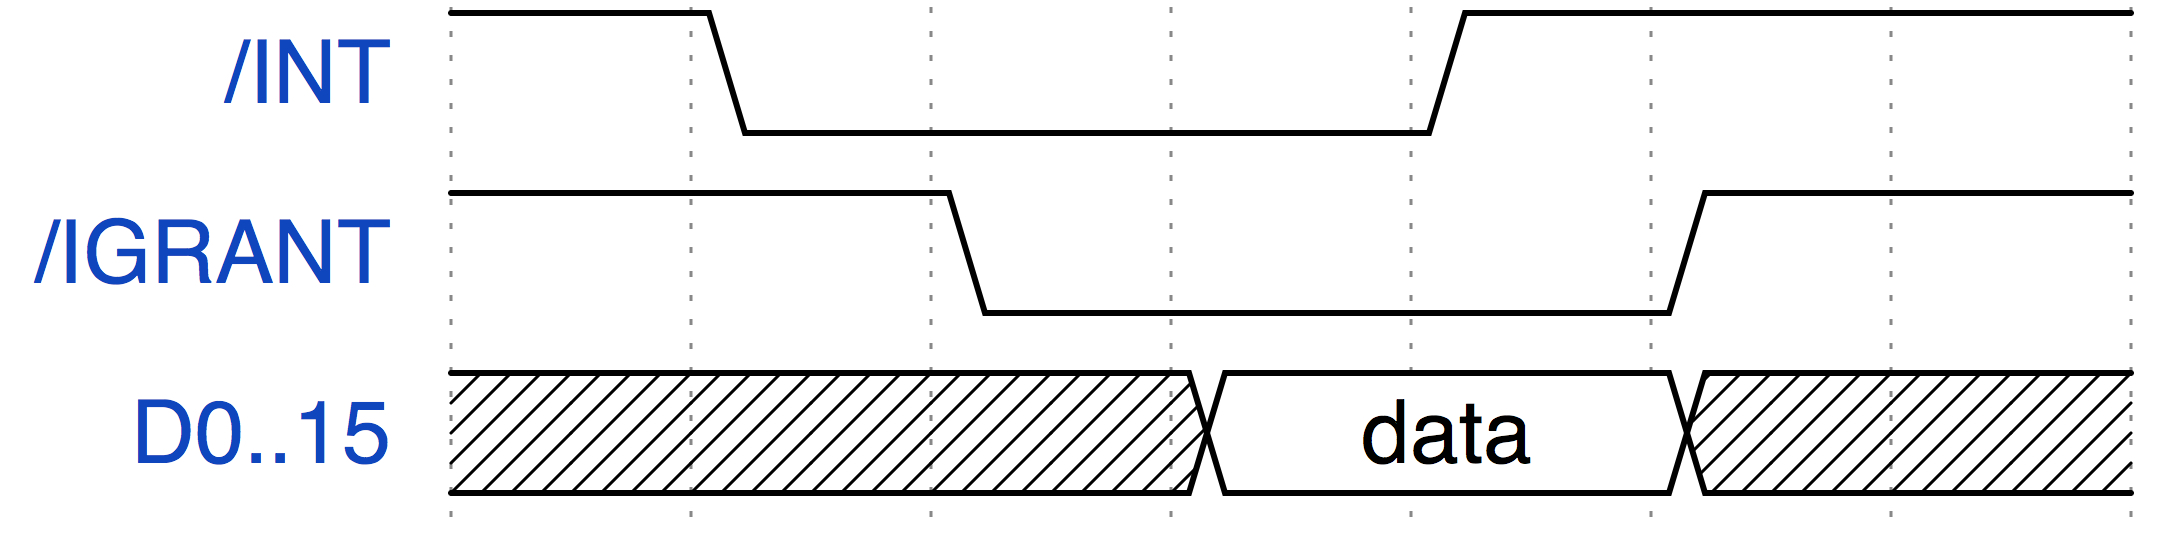
\includegraphics[width=.8\textwidth]{interrupt_timing.jpg}
   \end{center}
%https://wavedrom.com/editor.html:
%{signal: [
%  {name: '/INT', wave: '10..1..'},
%  {name: '/IGRANT', wave: '1.0..1.'},
%  
%  {name: 'D0..15', wave: 'xxx=.xx', data: ['data']},
%  
%]}
  \end{frame}
%
% \section{Soft- and hardware}
  \begin{frame}
   \frametitle{Soft- and hardware}
   \begin{itemize}
    \item The development suite for QNICE is available at 
     \texttt{http://qnice.sf.net}. It consists of an assembler and
     an emulator.
    \item The sources for Mirko Holzer's FPGA-implementation of
     QNICE can be found at \texttt{https://github.com/sy2002/QNICE-FPGA}.
     This repository also contains a copy of the necessary QNICE 
     software development utilities.
    \item Dr. \textsc{Chris Giles} currently (as of 2020) develops a
     microprogrammed TTL-implementation of the QNICE-architecture including
     interrupt handling.
   \end{itemize}
  \end{frame}
%
% \section{The emulator}
  \begin{frame}
   \frametitle{The emulator}
   \begin{itemize}
    \item The emulator is quite capable and not only implements
     the CPU but also some IO-devices such as a basic UART and
     an IDE-interface.
    \item It features a rich command set (\texttt{CB}, {\tt DEBUG}, {\tt DIS},
     {\tt DUMP}, {\tt HELP}, {\tt LOAD}, {\tt QUIT}, {\tt RESET}, {\tt RDUMP},
     {\tt RUN}, {\tt SET}, {\tt SAVE}, \texttt{SB}, {\tt STAT}, {\tt STEP}, 
     {\tt VERBOSE})
     and extensive statistical
     features which proved rather useful during the design and development
     of the instruction set and addressing modes.
   \end{itemize}
  \end{frame}
%
  \begin{frame}[containsverbatim]
   \frametitle{Using the emulator}
   \begin{description}
    \item [Load and disassemble the summation program:]
   \end{description}
   {\small
    \begin{verbatim}
Q> load sum.bin
Q> dis 0,9
Disassembled contents of memory locations 0000 - 0009:
0000: B000 XOR      R00, R00
0001: 0F84 MOVE     0x1000, R01
0002: 1000
0003: 1100 ADD      R01, R00
0004: 3F84 SUB      0x0001, R01
0005: 0001
0006: FF8B ABRA     0x0003, !Z
0007: 0003
0008: E000 HALT     
0009: 0000 MOVE     R00, R00
    \end{verbatim}
   }
  \end{frame}
%
  \begin{frame}
   \begin{description}
    \item [Show the register contents:]
   \end{description}
   {\tt
Q> rdump\\
Register dump: BANK = 00, SR = \_\_\_\_\_\_\_1\\
$\rule{0cm}{.1cm}$\\
        R00-R04: 0000 0000 0000 0000\\
        R04-R08: 0000 0000 0000 0000\\
        R08-R0c: 0000 0000 0000 0000\\
        R0c-R10: 0000 0000 0001 0000\\
   }
  \end{frame}
%
  \begin{frame}[containsverbatim]
   \begin{description}
    \item [Run the program and repeat the register dump:]
   \end{description}
   \begin{verbatim}
Q> run 
Q> rdump
Register dump: BANK = 00, SR = ____Z__1

    R00-R03: 0800 0000 0000 0000 
    R04-R07: 0000 0000 0000 0000 
    R08-R11: 0000 0000 0000 0000 
    R12-R15: 0000 0000 0009 0009 
   \end{verbatim}
  \end{frame}
%
  \begin{frame}[containsverbatim]
   \begin{description}
    \item [Print the statistics of this run:]
   \end{description}
   {\tiny
    \begin{verbatim}
Q> stat

20484 memory reads, 0 memory writes and
12291 instructions have been executed so far:

INSTR ABSOLUTE RELATIVE INSTR ABSOLUTE RELATIVE
-----------------------------------------------
MOVE:        1 ( 0.01%) ADD :     4096 (33.33%) 
ADDC:        0 ( 0.00%) SUB :     4096 (33.33%) 
SUBC:        0 ( 0.00%) SHL :        0 ( 0.00%) 
SHR :        0 ( 0.00%) SWAP:        0 ( 0.00%) 
NOT :        0 ( 0.00%) AND :        0 ( 0.00%) 
OR  :        0 ( 0.00%) XOR :        1 ( 0.01%) 
CMP :        0 ( 0.00%)     :        0 ( 0.00%) 
HALT:        1 ( 0.01%) ABRA:     4096 (33.33%) 
ASUB:        0 ( 0.00%) RBRA:        0 ( 0.00%) 
RSUB:        0 ( 0.00%) 

     READ ACCESSES                   WRITE ACCESSES
MODE   ABSOLUTE RELATIVE        MODE   ABSOLUTE RELATIVE
-----------------------------------------------------------
rx   :    12290 (42.86%)    rx   :     8194 (28.57%)
@rx  :        0 ( 0.00%)    @rx  :        0 ( 0.00%)
@rx++:     8193 (28.57%)    @rx++:        0 ( 0.00%)
@--rx:        0 ( 0.00%)    @--rx:        0 ( 0.00%)
    \end{verbatim}
   }
  \end{frame}
%
% \section{Future plans}
  \begin{frame}
   \frametitle{Future plans}
   \begin{itemize}
    \item As of now (AUG-2020) the following QNICE implementations 
     exist: 
     \begin{itemize}
      \item A software emulator (\texttt{qnice.c}),
      \item an AVR-implementation (only of historic interest),
      \item a \textbf{a fully fledged FPGA implementation}, and
      \item a TTL-implementation (ongoing project).
     \end{itemize}
    \item We plan to port a UNIX-like operating system such as 
     XINU to QNICE in the not too far future.
    \item A Forth-interpreter would be great, too. :-)
   \end{itemize}
  \end{frame}
%
 \begin{frame}
  \frametitle{Bibliography}
  \begin{thebibliography}{9}
   \bibitem{magic}
    Bill Buzbee's Magic Processor has been described extensively at 
    {\tt http://www.homebrewcpu.com}
   \bibitem{nice}
    Bernd Ulmann, \emph{NICE -- an elegant and powerful 32-bit architecture},
    Computer Architecture News, OCT-1997.
   \bibitem{nice_html}
    Bernd Ulmann, \emph{The NICE Processor Pages}, 
    {\tt http://www.vaxman.de/projects/nice/nice.html}
  \end{thebibliography}
 \end{frame}
\end{document}
